\documentclass{article}
\usepackage{graphicx} % Required for inserting images
% Useful packages for computer science thesis
\usepackage{amsmath}  % Advanced math formatting
\usepackage{amsthm}   % Theorem environments
\usepackage{algorithmic}  % Algorithm writing
\usepackage{algorithm}    % Algorithm floating environment
\usepackage{listings}     % Code listings
\usepackage{xcolor}       % Color support
\usepackage{caption}
\usepackage{multirow}
\usepackage{tikz}
\usepackage{amssymb}
\usepackage{booktabs}
\usepackage{subcaption}
\usepackage{booktabs}     % Professional tables
\usepackage{hyperref}     % PDF bookmarks and hyperlinks
\usepackage{cleveref}     % Smart cross-referencing
\usepackage{url}          % URL formatting

% Configure hyperref
\hypersetup{
    colorlinks=true,
    linkcolor=black,
    filecolor=magenta,
    urlcolor=[rgb]{0.0, 0.3, 0.7},
    citecolor=[rgb]{0.0, 0.5, 0.0}
}


\title{Data-Flow Analysis and Second Assignment}
\author{Andrea Lavino}
\date{March 2025}

\begin{document}

\maketitle

\clearpage

\tableofcontents

\clearpage

\section{Data-Flow Analysis}

Data-flow analysis is a set of techniques used to extract information from the intermediate representation code created by the compiler front-end. Extracting information is crucial task because, without knowledge about the program, the compiler won't be able to perform any optimization or at least not the complex ones.

Analysis can be performed both globally and locally. Local analysis focuses on the single basic block and its instructions, whereas global analysis focuses on the whole control flow graph and tries to understand the effects that each basic block has on the others. Data-flow analysis is a type of global analysis.

Before diving into some examples of the data-flow analysis problems, it is important to understand what are the effects that instructions and basic blocks can have. Finall, it is important to show the fundamental structure of a data-flow analysis problem and the common framework in which we operate when dealing with such problems.

\subsection{Instruction Effects}

Every instruction of the type $a = b + c$ can have three effects:

\begin{itemize}
    \item Uses: the instruction uses the variables $b$ and $c$ in order to compute the value of $a$
    \item Kills: the instruction kills a previous definition of $a$
    \item Defines: the instruction defines the variable $a$
\end{itemize}

The effects of every instruction compound creating the effect of the whole basic block

\subsection{Basic-Block Effects}

As the instructions, even a basic block can have three effects:

\begin{itemize}
    \item locally exposed use: the basic block uses a variable that it is not preivously defined within the BB, therefore uses a variable that was defined before the basic block entry point
    \item kills: every variable definition within the BB kills all the other definitions that have reached the basic block
    \item locally available definition: the basic block uses a variable that was previously defined in the same block
\end{itemize}

\subsubsection{Example}

Here there is a small example of the effects that a basic block can have.

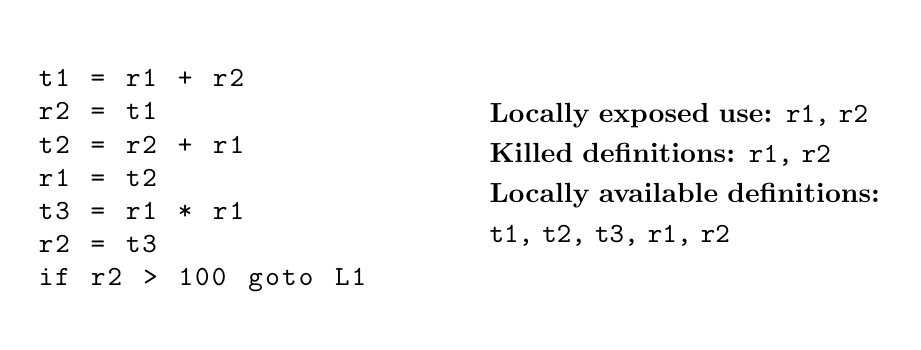
\begin{tikzpicture}
    \node[anchor=north west, text width=4cm] (code) {
\begin{lstlisting}[basicstyle=\ttfamily]
t1 = r1 + r2
r2 = t1
t2 = r2 + r1
r1 = t2
t3 = r1 * r1
r2 = t3
if r2 > 100 goto L1
\end{lstlisting}
    };

    % Add some text near the listing
    % Add some text near the listing with line-spacing
    \node[anchor=west, text width=5cm] at ([xshift=1.5cm]code.east) {
        \begin{minipage}{5cm}
            \baselineskip=1.2\baselineskip
            \textbf{Locally exposed use:} \texttt{r1, r2}
            \textbf{Killed definitions:} \texttt{r1, r2}
            \textbf{Locally available definitions:} \texttt{t1, t2, t3, r1, r2}
        \end{minipage}
    };


\end{tikzpicture}

\subsection{Data-Flow analysis problem structure}

 Each techique that lies in the domain of data-flow analysis aims at solving a specific problem regarding the gaining of knowledge about the program. Therefore, it is fundamental whenever we are approaching a data-flow analysis problem to clearly state our goal and define what we are trying to find about the program.

 After having properly defined the problem, it is important to define its transfer functions, i.e. the function that maps basic blocks inputs and its outputs and viceversa depending on the problem type (forward or backward).

 Besides the transfer function, other important elements that helps properly define the problem are the boundary and initial conditions of each basic block, the direction of the data flow (forward or backward) and the meet operator.

 All of the problem informations can be summarized using a simple table representation, like the following:

\begin{table}[H]
\centering
\begin{tabular}{|p{0.4\textwidth}|p{0.4\textwidth}|}
\hline
 & \textbf{Dataflow Problem X} \\
\hline
Domain & ? \\
\hline
Direction & ? \\
 & ? \\
 & ? \\
\hline
Transfer function & ? \\
\hline
Meet Operation ($\wedge$) & ? \\
\hline
Boundary Condition & ? \\
\hline
Initial interior points & ? \\
\hline
\end{tabular}
\caption{Generic data-flow problem table}
\label{tab:dataflow_problem_x}
\end{table}

\section{Reaching Definitions}

The problem of reaching definitions consists in finding all the available definitions in a specific point of the program. The information obtained by solving this problem can be used to check whether a variable is used before its definition.

\subsection{Problem formalization}

Formally we say that a definition \textit{d} reaches a point \textit{p} if there is a path from \textit{d} to \textit{p} where \textit{d} is not killed along the path.

\begin{table}[H]
\centering
\begin{tabular}{|p{0.4\textwidth}|p{0.4\textwidth}|}
\hline
 & \textbf{Reaching definitions problem} \\
\hline
Domain & Sets of definitions \\
\hline
Direction & Forward \\
 & $out[b] = f_b(in[b])$ \\
 & $in[b] = \wedge out[pred[b]]$ \\
\hline
Transfer function & $f_b(x) = Gen_b \cup (x - Kill_b)$ \\
\hline
Meet Operation ($\wedge$) & $\cup$ \\
\hline
Boundary Condition & $out[entry] = \varnothing$  \\
\hline
Initial interior points & $out[b] = \varnothing$  \\
\hline
\end{tabular}
\caption{Reaching Definition table summary}
\label{tab:dataflow_problem_x}
\end{table}

\subsection{Example}

\begin{figure}[H]
    \centering
    \begin{minipage}{0.45\textwidth}
        \includegraphics[width=\linewidth]{graphs/liveness_reaching.pdf}
    \end{minipage}%%
    \begin{minipage}{0.45\textwidth}
        \textbf{Description:} 
    \end{minipage}
    \caption{Reaching definitions problem example}
\end{figure}
\section{Liveness Analysis}

\subsection{Problem formalization}

\begin{table}[H]
\centering
\begin{tabular}{|p{0.4\textwidth}|p{0.4\textwidth}|}
\hline
 & \textbf{Dataflow Problem X} \\
\hline
Domain & ? \\
\hline
Direction & ? \\
 & ? \\
 & ? \\
\hline
Transfer function & ? \\
\hline
Meet Operation ($\wedge$) & ? \\
\hline
Boundary Condition & ? \\
\hline
Initial interior points & ? \\
\hline
\end{tabular}
\caption{Dataflow Problem X Properties}
\label{tab:dataflow_problem_x}
\end{table}

\subsection{Example}

\includegraphics[width=0.8\textwidth]{graphs/liveness_reaching.pdf}

\section{Available Expressions}

\subsection{Problem formalization}

\begin{table}[H]
\centering
\begin{tabular}{|p{0.4\textwidth}|p{0.4\textwidth}|}
\hline
 & \textbf{Dataflow Problem X} \\
\hline
Domain & ? \\
\hline
Direction & ? \\
 & ? \\
 & ? \\
\hline
Transfer function & ? \\
\hline
Meet Operation ($\wedge$) & ? \\
\hline
Boundary Condition & ? \\
\hline
Initial interior points & ? \\
\hline
\end{tabular}
\caption{Dataflow Problem X Properties}
\label{tab:dataflow_problem_x}
\end{table}

\subsection{Example}

\includegraphics[width=0.8\textwidth]{graphs/available_expressions.pdf}

\section{Very Busy Expressions}

\subsection{Problem formalization}

\begin{table}[H]
\centering
\begin{tabular}{|p{0.4\textwidth}|p{0.4\textwidth}|}
\hline
 & \textbf{Dataflow Problem X} \\
\hline
Domain & ? \\
\hline
Direction & ? \\
 & ? \\
 & ? \\
\hline
Transfer function & ? \\
\hline
Meet Operation ($\wedge$) & ? \\
\hline
Boundary Condition & ? \\
\hline
Initial interior points & ? \\
\hline
\end{tabular}
\caption{Dataflow Problem X Properties}
\label{tab:dataflow_problem_x}
\end{table}

\subsection{Example}

\includegraphics[width=0.8\textwidth]{graphs/very_busy.pdf}

\section{Dominator Analysis}

\subsection{Problem formalization}

\begin{table}[H]
\centering
\begin{tabular}{|p{0.4\textwidth}|p{0.4\textwidth}|}
\hline
 & \textbf{Dataflow Problem X} \\
\hline
Domain & ? \\
\hline
Direction & ? \\
 & ? \\
 & ? \\
\hline
Transfer function & ? \\
\hline
Meet Operation ($\wedge$) & ? \\
\hline
Boundary Condition & ? \\
\hline
Initial interior points & ? \\
\hline
\end{tabular}
\caption{Dataflow Problem X Properties}
\label{tab:dataflow_problem_x}
\end{table}

\subsection{Example}

\includegraphics[width=0.8\textwidth]{graphs/dominance.pdf}

\section{Constant Propagation}

\subsection{Problem formalization}

\begin{table}[H]
\centering
\begin{tabular}{|p{0.4\textwidth}|p{0.4\textwidth}|}
\hline
 & \textbf{Dataflow Problem X} \\
\hline
Domain & ? \\
\hline
Direction & ? \\
 & ? \\
 & ? \\
\hline
Transfer function & ? \\
\hline
Meet Operation ($\wedge$) & ? \\
\hline
Boundary Condition & ? \\
\hline
Initial interior points & ? \\
\hline
\end{tabular}
\caption{Dataflow Problem X Properties}
\label{tab:dataflow_problem_x}
\end{table}

\subsection{Example}

\includegraphics[width=0.5\textwidth]{graphs/constant_propagation.pdf}

\section{Interprocedural Summary Problems}

\subsection{Problem formalization}

\begin{table}[H]
\centering
\begin{tabular}{|p{0.4\textwidth}|p{0.4\textwidth}|}
\hline
 & \textbf{Dataflow Problem X} \\
\hline
Domain & ? \\
\hline
Direction & ? \\
 & ? \\
 & ? \\
\hline
Transfer function & ? \\
\hline
Meet Operation ($\wedge$) & ? \\
\hline
Boundary Condition & ? \\
\hline
Initial interior points & ? \\
\hline
\end{tabular}
\caption{Dataflow Problem X Properties}
\label{tab:dataflow_problem_x}
\end{table}

\subsection{Example}

\end{document}
